\documentclass[sigconf,anonymous]{acmart}
\usepackage{amsmath,booktabs,tikz}
\usetikzlibrary{positioning,arrows.meta,fit,backgrounds}
\setcopyright{none}
\settopmatter{printacmref=false}
\acmConference[TRUST '27]{ACM Conference on Trustworthy and Responsible AI and Computing Systems}{March 7--9, 2027}{Washington, DC, USA}
\acmYear{2027}
\acmDOI{}
\acmISBN{}
\title{Accountable Model Recovery for Blockchain-Assisted Federated Learning}
\author{Anonymous Author(s)}
\begin{document}
\begin{abstract}
Federated learning committees can approve harmful updates even when identities
are authenticated. Recording such approvals on a blockchain provides an audit
trail, but does not remove their effects from a learned model. We specify a
two-layer framework combining private local validation with accountable,
application-level model recovery. A rotating committee evaluates candidate
updates without pooling validation examples. A windowed monitor compares model
quality over time, and an append-only recovery transaction identifies an earlier
checkpoint and the affirmative signers associated with invalidated versions.
Enrollment uniqueness remains an external assumption, and quality reports are
attestations rather than cryptographic proofs of poisoning. The implementation
connects a reproducible federated-learning runner to Solidity contracts deployed
on a local EVM. We define matched evaluations on Fashion-MNIST and CIFAR-10,
including heterogeneous data, compromised validators, enrollment errors, and
ablation studies. Confirmatory robustness results remain pending; the present
draft reports implementation validation separately from scientific evidence.
\end{abstract}
\ccsdesc[500]{Security and privacy~Distributed systems security}
\ccsdesc[300]{Computing methodologies~Machine learning}
\keywords{federated learning, model poisoning, accountability, blockchain, recovery}
\maketitle
\begin{center}
\fbox{\parbox{0.95\columnwidth}{\textbf{Working research draft.}
Core, SIFT and follow-up experiments are incomplete.
This PDF is not yet ready for submission.}}
\end{center}
\section{Introduction}
Federated learning distributes model training while retaining examples at
participating clients~\cite{mcmahan2017}. Its aggregation interface also gives
compromised participants a direct mechanism for modifying the global model.
In decentralized settings, the aggregation policy must additionally determine
who can participate, how updates are validated, and what happens after harmful
updates have been accepted.

Enrollment, robust aggregation, private evaluation, and recovery have distinct
trust boundaries. An enrolled participant can be malicious, heterogeneous data
can violate aggregation assumptions, and a ledger cannot establish the correctness
of private evaluations. Restoring model parameters also leaves earlier approval
transactions intact.

We study a two-layer architecture that makes these boundaries explicit. Layer~1
uses enrolled, staked validators to assess candidate updates on private local
validation data. Layer~2 monitors model quality and records checkpoint restoration
and attributed penalties. The ledger remains append-only throughout recovery.
The term \emph{accountable} denotes recorded responsibility and enforceable stake
accounting under the stated trust assumptions; it does not imply that a negative
quality trend proves malicious intent.

The intended contribution is an executable system specification with observable
failure boundaries: exact committee and quorum rules, disjoint validation and
test data, recovery that preserves blockchain history, and separate measurements
of malicious-update acceptance, downstream attack success, and wrongful penalties.
Component ablations and matched aggregation baselines evaluate the integrated
mechanism. EMH-DNN routing is a secondary case study. Robustness claims require
completed, matched-seed experiments.

\section{Related Work}
\paragraph{Robust aggregation and heterogeneity.}
FedAvg aggregates data-weighted local updates~\cite{mcmahan2017}.
Krum selects updates using inter-update distances~\cite{blanchard2017};
coordinate median uses coordinate-wise order statistics~\cite{yin2018}.
FLTrust introduces a trusted server reference update and combines directional
alignment with norm normalization~\cite{cao2021}. BOBA addresses label skewness
through robust affine-subspace estimation and label-distribution
filtering~\cite{bao2024}. Their assumptions differ: the proposed committee has
private validation examples, while FLTrust and BOBA receive designated trusted
reference examples. These differences are reported alongside results instead of
being hidden in a single robustness ranking.
FedVal scores updates using server validation losses and balances class-level
performance~\cite{valadi2023}. This is a particularly relevant comparator:
private committee validation changes the location and distribution of the
reference information, but does not by itself establish fairer evaluation.
Our follow-up implementation uses the published scoring rule and records
differences from the released software. Recent theoretical work studies
cooperative identification of data-poisoned workers~\cite{yu2026}; its assumptions
do not directly supply guarantees against arbitrary submitted model updates.

\paragraph{Detection and adaptive backdoors.}
FLDetector identifies clients whose updates repeatedly disagree with predictions
from their update history~\cite{zhang2022detector}. Our monitor tracks committee
utility trends without identifying a poisoning client. FLAME combines
clustering, clipping and noise for backdoor
defense~\cite{nguyen2022flame}. Model replacement and constrain-and-scale attacks
demonstrate why maintaining clean accuracy can coexist with a harmful
backdoor~\cite{bagdasaryan2020}. Consequently, neither a reversed-update ramp
nor untargeted accuracy degradation alone evaluates adaptive evasion. Our
follow-up search uses attacker-owned proxy examples and a clean-utility
constraint; it is a bounded attack, not an optimal-adversary guarantee.

\paragraph{Blockchain-assisted learning.}
Biscotti combines a ledger with privacy and robustness mechanisms~\cite{shayan2022}.
Recent work also studies verification of local training and aggregation:
VerifBFL uses zk-SNARKs and incrementally verifiable computation and includes
differential privacy~\cite{bellachia2025}. Our local-EVM prototype makes a weaker
verification claim. Its contracts enforce authorization, vote uniqueness, quorum,
and stake transitions; they do not verify numerical training or privately
computed quality reports. Consequently, neither raw-data locality nor a hash
commitment is described as a formal privacy guarantee.

\paragraph{Recovery after poisoning.}
FedRecover uses historical information to reduce recovery
costs~\cite{cao2023recover}. Crab investigates efficient and certified
recovery~\cite{jiang2024}. The 2026 FAUN preprint uses adversarial unlearning
and a short history of malicious updates~\cite{zhao2026}.
Our recovery operation restores a historical checkpoint, preserves ledger history,
and attributes responsibility to recorded approvals. It provides neither certified
unlearning nor a guarantee that the restored checkpoint is clean. These recovery
methods motivate explicit measurements of residual damage and recovery cost;
their reported numbers are not transferred into our experimental tables.
We therefore compare continuing training with plain restoration and restoration
with attributed penalties under the same prespecified intervention time and
checkpoint. These controls isolate the consequences of restoration and sanctions;
they are not implementations of FedRecover or Crab.

\section{Threat Model and Assumptions}
\label{sec:threat}
There are $N$ enrolled client accounts. Some control unique identities; others
may represent duplicate enrollment attempts. A trusted external registrar models
identity uniqueness with configurable false-accept and false-reject rates.
The prototype does not implement biometric, social-graph, or other
Proof-of-Personhood verification. Independently enrolled colluding participants
therefore remain in scope even when enrollment makes no errors.

The adversary can poison local updates and independently compromise validators.
Corrupted validators may approve poisoned updates, reject honest updates, or
report inflated monitoring quality. The experiment driver knows attacker labels
for injection and scoring. Honest validation, eligibility, aggregation, and
recovery do not receive these labels. ALIE experiments assume access to honest
reference updates and are labeled as an omniscient-adversary setting.

The registrar, off-chain experiment orchestrator, model aggregation computation,
and checkpoint store are trusted. The ledger authenticates account transactions
and enforces its contract state machine. It does not prove that a reported score
was obtained from an authentic validation partition. In particular, a malicious
majority or a biased committee can defeat the quality monitor.

Client data is divided into disjoint training and private validation partitions.
Held-out test examples are used exclusively for reporting. Trusted server
reference examples are reserved separately for methods that require them, and
are removed from all client partitions. Raw validation examples remain local;
model updates and released metrics may still leak information. Secure aggregation,
differential privacy, and a production identity service are outside this
implementation's guarantees.

\section{Two-Layer Validation and Recovery}
\label{sec:framework}
\begin{figure}[t]
\centering
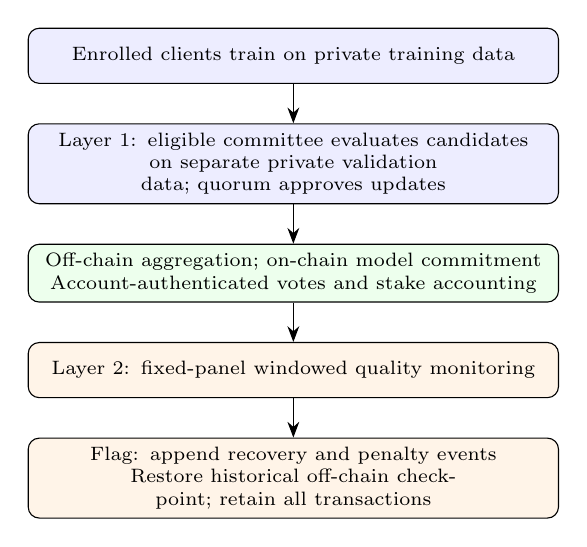
\begin{tikzpicture}[node distance=5mm,font=\scriptsize,
box/.style={draw,rounded corners,align=center,text width=6.5cm,minimum height=7mm},
arr/.style={-{Stealth[length=2mm]}}]
\node[box,fill=blue!7] (train) {Enrolled clients train on private training data};
\node[box,below=of train,fill=blue!7] (vote) {Layer 1: eligible committee evaluates candidates\\on separate private validation data; quorum approves updates};
\node[box,below=of vote,fill=green!7] (commit) {Off-chain aggregation; on-chain model commitment\\Account-authenticated votes and stake accounting};
\node[box,below=of commit,fill=orange!9] (monitor) {Layer 2: fixed-panel windowed quality monitoring};
\node[box,below=of monitor,fill=orange!9] (recover) {Flag: append recovery and penalty events\\Restore historical off-chain checkpoint; retain all transactions};
\draw[arr] (train)--(vote);\draw[arr] (vote)--(commit);
\draw[arr] (commit)--(monitor);\draw[arr] (monitor)--(recover);
\end{tikzpicture}
\caption{System workflow. Raw examples remain local. The contracts enforce
protocol transitions; they do not verify private quality measurements.}
\Description{Five vertically connected steps: client training, private committee validation, model commitment, quality monitoring, and append-only recovery.}
\label{fig:system}
\end{figure}

\subsection{Layer 1: Eligibility and Validation}
For candidate client $k$, let $E$ be the number of eligible validators after
excluding $k$. Enrollment, minimum stake, and the configured trust threshold
determine eligibility. The committee size and approval threshold are
\begin{equation}
 C=\min\{E,\max\{3,\lceil0.3E\rceil\}\},\qquad
 q=\lceil2C/3\rceil.
\end{equation}
When $E<3$, validation is unsupported; it is never replaced with a one-member
committee. For example, four enrolled eligible clients give a three-member
committee after excluding the proposer and require two affirmative votes.
Each candidate receives an independently sampled committee with a reproducible
random stream. Committees are sampled independently of participant selection.

Validator $j$ evaluates the candidate and current model on the same private
validation partition. With utility $u_j$, its normalized change is
\begin{equation}
 d_{jk}=\frac{u_j(w+\Delta_k)-u_j(w)}{\max\{|u_j(w)|,10^{-12}\}}.
\end{equation}
The default approval rule is $d_{jk}\geq-0.05$. A candidate requires $q$
distinct affirmative signers; repeated votes cannot increase support.
The median normalized change is recorded diagnostically and is not substituted
for quorum. Accepted updates are aggregated as
\begin{equation}
 w'=w+\frac{\sum_{k\in A} n_k\tau_k\Delta_k}{\sum_{k\in A}n_k\tau_k},
\end{equation}
where $A$ is the approved set, $n_k$ is its training sample count, and $\tau_k$
is recorded trust. Empty or unsupported approval sets produce explicit no-op
rounds. Trust changes follow recorded approval or rejection outcomes, with
additional penalties after recovery. They do not use ground-truth attacker labels.
Trust starts at $0.5$; validator eligibility requires $\tau_k\geq0.45$, while
candidate training stops below the floor $0.15$. Approval adds $0.02$ trust;
rejection or a recovery-attributed penalty subtracts $0.15$, clipped to $[0,1]$.
Initial stake is 20 credits, eligibility requires 10, and an attributed penalty
deducts five. These are prespecified starting values rather than theoretically
optimal thresholds. Eligibility sensitivity includes $0.30$, $0.45$, and $0.50$;
its outcomes are needed to justify a final deployment choice.

\subsection{Layer 2: Monitoring a Fixed Panel}
A panel is fixed for a window of five observations, including the baseline
before its first candidate round. Panel members evaluate consecutive versions
on their private validation partitions. Keeping panel membership constant within
the window reduces score changes caused solely by resampling validators.
Let $s_i$ be the median panel utility at observation $i$. With $W=5$, the monitor
compares the latest score with the mean of preceding window scores and fits
a least-squares linear slope:
\begin{equation}
 D=\frac{\overline{s}_{1:W-1}-s_W}{\max\{|\overline{s}_{1:W-1}|,10^{-12}\}}.
\end{equation}
A relative drop above $0.05$ or a slope below $-0.005$ triggers recovery.
An adjacent-round detector is evaluated separately. Thresholds are prespecified
and their sensitivity is measured using development seeds. Non-IID data and benign
drift can trigger both monitors, so detection does not prove an attack occurred.

\subsection{Append-Only Recovery and Accountability}
Every model version has a commitment, parent pointer, and off-chain checkpoint.
After a flagged window, recovery restores the checkpoint preceding that window.
The contract appends the invalidated interval, restored version, monitoring-panel
attestations, and penalty events. Earlier commitments remain retrievable.
The restored checkpoint is historical and may contain older poisoning.

Only affirmative signers of commitments in the invalidated interval are eligible
for penalties. A signer is penalized at most once per recovery event. Rejected
votes and nonparticipants are not penalized. Stake and trust changes persist after
model restoration; the detector history resets and a new panel is selected.
Because honest signers can approve harmful updates or a monitor can misfire,
wrongful penalties are a primary outcome rather than an omitted corner case.

\section{Implementation and Complexity}
\label{sec:implementation}
The Python runner implements deterministic data partitions, separate random
streams, batched evaluation, and CPU or CUDA training. Each run preserves its
configuration, content fingerprints, split indices, JSONL event log, model-version
trace, and summary. Completed runs are immutable. Interrupted seeds are restarted
into fresh directories while retaining the earlier logs.

Solidity contracts are compiled with optimization and deployed to a persistent
local Hardhat EVM. Account transactions authenticate votes. Candidate identifiers
bind the chain, contract, experiment, round, base version, proposer, and update
hash. The contract checks enrollment, stake, proposer exclusion, distinct
committee members, vote uniqueness, and quorum. Recovery requires a quorum of
panel attestations. The experiment orchestrator remains responsible for selecting
the committee and computing model aggregation.

For each transaction, the adapter records its receipt, gas used, calldata size,
and local elapsed time. These are measured execution costs on a development chain,
not estimates of public-network confirmation latency. Stake credits use a fixed
conversion of one credit to $10^9$ wei for reproducible accounting; this arbitrary
unit does not establish an economic incentive model.

If $P$ clients participate, $C$ validators assess each candidate, and model updates
contain $d$ scalars, candidate distribution requires $O(PCd)$ transmitted scalar
values, plus model broadcast and monitoring reports. Validation can dominate
training when many committees repeatedly evaluate candidates. On-chain candidate
snapshots and votes grow as $O(PC)$ per round. Recovery scans the flagged interval
and its affirmative signers. Local execution of those loops does not demonstrate
that all intervals fit production gas limits.

\begin{figure}[t]
\centering
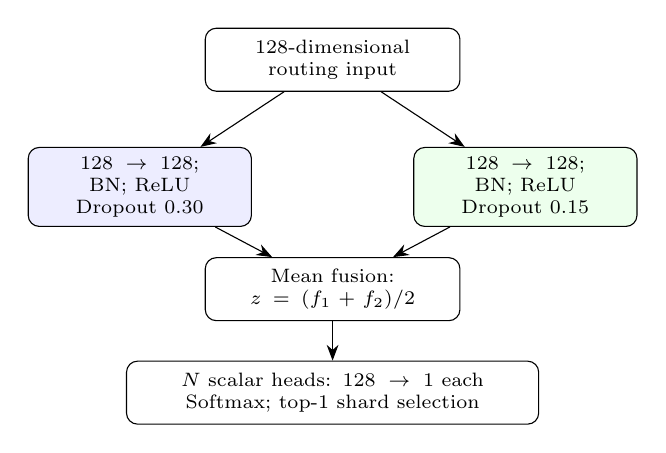
\begin{tikzpicture}[node distance=5mm,font=\scriptsize,
box/.style={draw,rounded corners,align=center,minimum height=8mm},
arr/.style={-{Stealth[length=2mm]}}]
\node[box,text width=3cm] (input) {128-dimensional routing input};
\node[box,below left=7mm and -6mm of input,text width=2.6cm,fill=blue!7] (a) {$128\rightarrow128$; BN; ReLU\\Dropout 0.30};
\node[box,below right=7mm and -6mm of input,text width=2.6cm,fill=green!7] (b) {$128\rightarrow128$; BN; ReLU\\Dropout 0.15};
\node[box,below=21mm of input,text width=3cm] (fusion) {Mean fusion: $z=(f_1+f_2)/2$};
\node[box,below=of fusion,text width=5cm] (heads) {$N$ scalar heads: $128\rightarrow1$ each\\Softmax; top-1 shard selection};
\draw[arr] (input)--(a);\draw[arr] (input)--(b);
\draw[arr] (a)--(fusion);\draw[arr] (b)--(fusion);\draw[arr] (fusion)--(heads);
\end{tikzpicture}
\caption{EMH-DNN supporting routing model. Both branches receive the complete
input; client heads add $129N$ parameters.}
\Description{A 128-dimensional input feeds two parallel neural branches with different dropout rates, then mean fusion and one scalar head per shard.}
\label{fig:emh}
\end{figure}

The routing case study uses two parallel $128$-unit branches, complementary
dropout rates of $0.30$ and $0.15$, mean fusion, and one scalar output per shard.
The input contains 128 dimensions. With $N$ shards, the output heads add $129N$
parameters; this linear growth is measured separately from the security protocol.
No architectural convergence or catastrophic-forgetting guarantee is claimed.

\section{Experimental Protocol}
\label{sec:evaluation}
\paragraph{Questions.}
We evaluate how the framework changes clean utility and attack damage, whether
windowed monitoring detects gradual degradation, how enrollment errors and
committee capture change outcomes, and what communication and contract costs
the additional mechanisms introduce.

\paragraph{Core experiment.}
Fashion-MNIST and CIFAR-10 use their official held-out test sets. Client training
and private validation are partitioned from the official training pool after
removing the common reserved reference pool. Defaults are 50 clients, 40\%
participation, 100 rounds, one local epoch, batch size 64, learning rate 0.01,
Dirichlet $\alpha=0.5$, and 30\% poisoning clients. Small empty shards are repaired
deterministically to retain separate training and validation examples.

The six methods are FedAvg, coordinate median, Multi-Krum, FLTrust, BOBA, and the
two-layer framework. The five conditions are clean, sign flip, ALIE, targeted
model replacement, and gradual poisoning. Confirmatory seeds are
$\{13,29,47,71,101\}$; development uses $\{3,5,7\}$. The core matrix therefore
contains 300 seed-level runs. Participants, partitions, initial models, and
training random streams are matched across methods. Trusted-reference assumptions
and infeasible Byzantine bounds are reported explicitly.
The core uses a controlled participation budget: each round samples a fixed
poisoning-client quota without replacement and fills the remaining slots from
honest enrolled accounts. This experimental schedule supplies no attacker labels
to the defense. It prevents uniform sampling fluctuations from silently exceeding
the declared Byzantine budget. Uniform sampling remains available separately;
its bound violations are reported as assumption failures.

\paragraph{Attack checks.}
Sign flip negates local deltas; ALIE replaces a malicious update with the
coordinate mean plus standard deviation of honest reference updates. This fixed
$z=1$ omniscient variant is motivated by ALIE~\cite{baruch2019}; it is not a
reproduction of every parameter choice in that work. Model
replacement combines local trigger poisoning with participant-to-attacker norm
scaling. Gradual poisoning interpolates from an honest update toward a reversed
update over ten rounds, with norm bounded by 1.5 times the original norm.
Before confirmatory execution, untargeted attacks require positive mean damage
on three development seeds against FedAvg. Targeted attacks require increased
trigger success over a clean model evaluated with the identical trigger.
Ineffective attacks are recorded and held for revision rather than presented as
successful defenses.

\paragraph{Sensitivity and ablations.}
Fashion-MNIST studies vary population $N\in\{20,50,80\}$, IID versus Dirichlet
$\alpha\in\{1,0.5,0.1\}$, and poisoning fractions 10\%, 30\%, and 50\%.
Independent validator capture and nonzero duplicate attempts exercise the
identity assumptions. The ablations remove recovery, remove penalties, or replace
windowed detection with adjacent-round comparison. Benign training-distribution
shifts and threshold sweeps test false alarms. Held-out evaluation shards are
used for worst-client utility; private validation scores are not reused as test
measurements.

\paragraph{Metrics and uncertainty.}
We distinguish malicious-update acceptance from targeted attack success.
Reported outcomes include final utility, learning-curve area, attack-induced
utility loss, utility before and after recovery, attack-presence detector FPR/FNR,
detection delay, recovery count, worst-client utility, wrongful penalties,
runtime, transmitted bytes, and ledger growth. A detector true positive denotes
a flag during a round containing an attack; it does not prove causal attribution.
Seed-level bootstrap intervals and paired differences are used; rounds are not
independent replicates. Prespecified paired tests use Holm correction.

\paragraph{New SIFT1M routing case study.}
The original project's custom shard labels have unverifiable provenance and
are excluded. The replacement uses the public SIFT1M archive: a database of
one million 128-dimensional descriptors, 100,000 learning queries, and 10,000
held-out queries~\cite{faisssift}. We recompute exact top-1000 neighbors on the
database for both query sets using CPU FAISS IndexFlatL2. Sampled neighbor results
and the published ground truth are checked using independent exhaustive
float64 distance calculations. Four- and eight-shard partitions are generated
from database vectors with centroid clustering, seed 2027 and 25 iterations.
Each target counts actual neighbor IDs in these recorded partitions; every
target row sums to 1000. Both query sets are scaled by 255, and EMH-DNN and MLP
use the same top-1 shard budget. Archive and generated-array checksums preserve
the data lineage. These are new SIFT1M experiments and cannot reproduce the
earlier shard labels or establish billion-vector performance. Three development
seeds screen attacks before the five-seed case-study matrix. SIFT runs use CPU
while the classification study runs separately; concurrent wall-time measurements
are exploratory rather than isolated overhead measurements.

\paragraph{Follow-up study.}
A separate implementation adds paper-based FedVal, natural-client FEMNIST,
adaptive attacks and recovery controls. Its 33 development runs precede up to
275 evaluation runs, each comparison requiring the five confirmatory seeds.
The original core and this extension have separate source fingerprints and
must not be pooled as one implementation. In particular, the extension requires
local degradation attestations from at least $\lceil2C/3\rceil$ members of the
fixed monitoring panel before applying a trend-triggered recovery. It records
the full panel and actual attesters separately. Evidence for this strengthened
recovery policy is pending; the earlier core cannot establish its robustness.

FEMNIST uses the official 62-class TensorFlow Federated distribution derived
from LEAF, with 50 writer clients per seed~\cite{tfffemnist}. The archive hash
matches the checksum in the official loader. Reference examples come from
different writers and cover every class. Enrolled writers retain their official
held-out test examples; their training data is split into training and private
validation. Exact pixel duplicates are removed from training and reference data,
including matches to test images, before those partitions are formed. Test
labels are not used in deduplication. The manifest records writer selection,
removed duplicates, per-client counts and all generated-file hashes. We report
lower-decile utility and exclusion rates alongside worst-client utility; these
writer-level measurements do not establish demographic fairness.

Matched Fashion-MNIST and FEMNIST comparisons use FedAvg, FLTrust, FedVal,
validation only and the full extension. Targeted adaptive evaluation on
Fashion-MNIST searches eight update scales using only attacker-owned training
examples and the public model. A candidate must retain proxy clean accuracy
within 0.02 absolute and have norm at most 1.5 times the attacker's benign update.
This search is validated against FedAvg before defense comparisons. Its proxy
constraints do not guarantee evasion of honest private validation.

Recovery-only controls fix the attack start at round 6, restoration decision at
round 20, and checkpoint at round 5. Continuing training, plain restoration and
restoration with penalties share their histories before intervention. This is a
controlled comparison with a prespecified historical checkpoint, distinct from
end-to-end detection. Additional stress tests independently corrupt 0\%, 30\%
or 70\% of validators for false recovery reports, and 30\% or 70\% for vote
withholding. Uniform participation separately exposes sampled Byzantine-bound
violations. The first completed full-framework development trace is replayed on
the EVM with active-version and final-stake agreement checks. Runtime estimates
from concurrent CPU preflight runs guide scheduling and do not establish
isolated overhead or public-network latency.

\section{Results and Evidence Status}
\label{sec:results}
As of the latest artifact generation, 294 of 300 core seed-level runs have completed. 58 comparison cells contain all five confirmatory seeds. Incomplete cells are excluded from numerical estimates.

\begin{table}[t]\centering\caption{Measured local-EVM implementation check (five synthetic rounds). These are not robustness results.}
\begin{tabular}{lr}\toprule Measurement & Value \\ \midrule
Transactions (including setup) & 47 \\
Total gas used & 7,790,575 \\
Total calldata bytes & 12,086 \\
\bottomrule\end{tabular}\label{tab:contract}\end{table}

\begin{table}[t]\centering\caption{Complete five-round synthetic development traces replayed on the local EVM. Totals include deployment and enrollment; each population has one trace.}
\begin{tabular}{rrr}\toprule Clients & Transactions & Total gas \\ \midrule
20 & 327 & 52,344,109 \\
50 & 1,707 & 257,943,763 \\
80 & 4,167 & 618,744,834 \\
\bottomrule\end{tabular}\label{tab:scaling}\end{table}

\begin{figure*}[t]\centering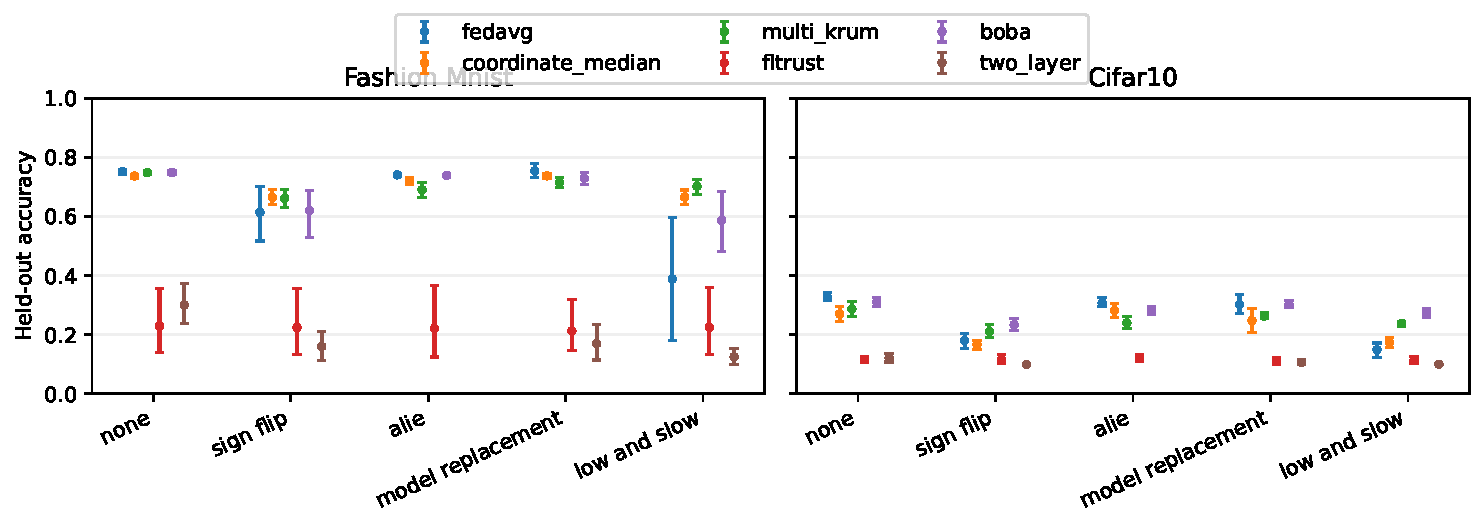
\includegraphics[width=0.95\textwidth]{figures/core_accuracy.pdf}
\caption{Matched core evaluation. Points show five-seed mean held-out accuracy; bars show bootstrap 95\% confidence intervals. Missing cells are incomplete or held, not zero-valued.}
\Description{Two dataset panels comparing complete five-seed groups across five attack conditions.}
\end{figure*}

\paragraph{Follow-up evidence status.}
No complete five-seed follow-up group is available. FedVal, FEMNIST, adaptive-attack and recovery-control results remain pending.

Implementation tests and local-EVM transactions establish execution of the
specified state machine. They do not establish robustness under real data,
large-scale Byzantine tolerance, privacy, or economic deterrence. The original
four/eight-client pilot and earlier synthetic diagnostics are excluded from
confirmatory tables. Completed development experiments are also excluded from
the confirmatory estimates.
The FedVal/FEMNIST extension is also pending. Its strengthened recovery
attestation rule is a protocol change, so original core outcomes are not
presented as validation of that rule. No result from a one-round runtime
preflight is included in robustness estimates.

The matched comparison table replaces cross-paper numerical rankings. Entries
are generated only after all five seeds for a cell have completed. Missing or
infeasible cells remain identifiable in the artifact status report. No zero-ASR
or zero-loss conclusion is drawn from a final-round acceptance counter.

\section{Limitations and Responsible Use}
Private validation partitions can differ systematically across clients, so median
quality is not an unbiased estimator of global utility. Fixed-panel monitoring
reduces one source of score variation but cannot distinguish every benign drift
from poisoning. Detector error rates and utility before and after recovery must be
interpreted together.

Checkpoint restoration can lose useful progress and leave earlier poison intact.
Wrongful penalties can exclude honest validators and reduce future committee
availability. Stake requirements also create participation barriers. These effects
limit any claim that staking alone makes an attack unprofitable. A utility model
and strategic-adversary analysis would be needed for such a claim.

The local EVM provides contract execution and transaction receipts on one host.
It does not measure network partitions, distributed consensus, adversarial block
production, or production checkpoint availability. The trusted registrar and
orchestrator are material deployment assumptions. Metric releases and individual
model updates retain privacy risks, and an anonymous deployment would require a
separate enrollment mechanism.

Classification findings require separate validation for search routing.
The new SIFT1M labels have explicit provenance, but the case-study outcomes
remain pending. Their sharding differs from the original pilot, so numerical
comparisons with its reported recall would be invalid.

\section{Conclusion}
The framework combines committee validation with recorded responsibility and
append-only recovery transactions. It separates validation from testing and
connects model-version traces to deployed Solidity contracts. Local execution
checks establish implementation behavior. Robustness, recovery benefit,
non-IID fairness, and scale remain questions for the matched evaluations.

\section*{GenAI Usage Disclosure}
An AI coding assistant was used to assist with implementation changes, experiment
orchestration, literature discovery, manuscript drafting, and figure construction.
The authors must review the implementation, verify citations and experimental
artifacts, and accept responsibility for the final manuscript. This statement
describes the assistance used during preparation and must be reviewed by the
authors before submission.
\bibliographystyle{ACM-Reference-Format}
\bibliography{references}
\end{document}
